%!TEX root=../documentation-bachlorthesis-speicherarchitektur-lstucker.tex
\cleardoublepage
\chapter{Speicherarchitekturen}

Die heutigen Speicherarchitekturen können in Block- (Block-Based), Datei- (File-Based) und Objekt-Basierende adressierende Systeme unterteilt werden.

\section{Block-Basierend}
Die Block-Basierende Speicherarchitektur ist wohl die traditionellste und weit verbreitetste Form zum Speichern und Zuzugreifen von Daten. Die meisten Computersysteme, sei es Server, Desktop-PCs, Tablet-PC, Smartphones, Spielkonsole, speichern Ihre Daten in einen Blockbasierenden Speicher ab. Als Speicher werden in diesen Geräte meist magnetischen Festplatten, Solid State Disk oder Flash-Speicher eingesetzt.

Bei Block-Speicher werden Daten in Blöcke gelesen und gespeichert (adressiert), ein Block bildet sich aus einer Sequenz von Bits bzw. Byte. Die Grösse eines Blocks wird als Blocklänge bezeichnet, und ist bei allen Blöcken einer Einheit gleich gross. 

Experten wie Mike Mesnier, Greg Ganger und Erik Riedel, sehen jedoch bei zunehmender Speichergrösse und Komplexität von Systemen fundamentale Limitierungen von Block Schnittstellen.

\begin{quotation}
\em Since the first disk drive in 1956, disks have grown by over six orders of magnitude in density and over four orders in performance, yet the storage interface (i.e., blocks) has remained largely unchanged. Although the stability of the block-based interfaces of SCSI and ATA/IDE has benefited systems, it is now becoming a lim- iting factor for many storage architectures. As storage infrastructures increase in both size and complexity, the functions system designers want to perform are fundamentally limited by the block interface. \end{quotation}\cite{Mesnier2003}

Vergleicht man die erste Festplatte, welche von IBM produziert wurde, mit einer Seagate von 2011, hat sich die Speicherdichte von 2000 bit per Quadratzoll auf 625 Gigabyte und in der Geschwindigkeit von 8 Kilobyte auf 600 Megabyte verbessert\cite{Seagate2011}\cite{Seagate2011a}

Für den Zugriff auf Blockbasierende Speichersysteme werden meist Schnittstellen Protokolle wie Small Computer System Interface (SCSI) oder Advanced Technology Attachment (ATA) verwendet. Diese Protokolle wurden jedoch in einer Zeit entwickelt, wo man davon ausging, dass ein Block Speicher jeweils nur von einem Computersystem verwendet wurde und nicht mit mehreren Computersystemen geteilt wird. Dies Annahme stimmt in Consumer Elektronik Bereich meist noch heute, in Bereichen wo jedoch grosse Speicherkapazitäten oder eine grössere Verfügbarkeit gefordert ist, wie Sie im Geschäftsbereich vorkommen, stimmen diese Annahmen nicht mehr.

Blockbasierende Speicher, welche nicht aus Internen Speicher eines Server gebildet werden, unterscheidet man in Direct Attached Storage (DAS) und Storage Area Network (SAN). 

\subsection{Direct Attached Storage}
Bei DAS handelt es sich, wie es aus der englischen Bezeichnung zu entnehmen ist, um Speicher, welche direkt an ein Computersystem angeschlossen wird. Bei DAS Enclosure handelt sich um ein Gehäuse mit mehren verbauten Festplatten, welche üblich über einen Host-Bus-Adapter an ein Computersytem angeschlossen wird. Als Schnittstellen Protokoll werden ATA, STA, eSATA, SCSI, SAS und Fibre Channel eingesetzt. DAS können mit mehreren Computersystemen geteilt werden, sofern genügen Schnittstellen zur Verfügung stehen.

\subsection{Storage Area Network}
Die Storage Networking Industry Association (SNIA) definiert ein Storage Area Network (SAN) als ein Netzwerk, welch primärer Bestimmungszweck ist Daten zwischen Computersysteme und Speicherelemente und unter Storage Elemente zu transferieren. Ein SAN besteht aus einer Kommunikations-Infrastrukture, welches eine physische Verbindung und eine Management-Schicht beinhaltet, welches die Verbindungen, die Speichereinheiten und das Computersystem organisiert, sodass der Datentransfer sicher und robust erfolgen kann. Der Begriff SAN wird normalerweise (aber nicht notwendigerweise) mit dem Block I/O Service in Verbindung gebracht und weniger mit dem Datei-Zugriff-Service.\cite{SNIA2011}

Je nach SAN Implementierung kommen folgende Geräte bzw. Komponenten vor:
\begin{itemize}
\item Server
\item Host Bus Adapter
\item Gigabit Interface Converter
\item SAN-Switch
\item Speichersystem
\item Tape Library
\item Logical Unit
\end{itemize}

\paragraph*{Server} 
Der Server greift über das SAN auf Ressourcen von Speichersystem oder Tape Library. In einzelnen Fällen kann der Server selbst über SAN anderen Server Speicher zur Verfügung stellen.

\paragraph*{Host Bus Adapter}
Host Bus Adapter (HBA) für das SAN sind intelligente Hardwareschnittstellen, welche für die Verbindung von Server in einem SAN verwendet werden. Sofern die Server nicht bereits mit einen Host Bus Adapter ausgerüstet sind, können die meisten durch Host Bus Adapter in form von Steckkarten erweitert werden. Der Host Bus Adapter selber hat pro Port ein Einschub in welche ein Gigabit Interface Converter eingebaut wird. \cite{Christopher2009}

\paragraph*{Gigabit Interface Converter}
Der Gigabit Interface Converter sind modulare Schnittstellen, welche Elektrische Signale in optische Signale umwandeln.\cite{SNIA2011}

\paragraph*{SAN-Switch}
Der SAN Switch ist ein Switch, welche dezidiert für das SAN Umgebung verwendet wird.

\paragraph*{Speichersystem}
Das Speichersystem stellt im SAN den geteilten Speicher zur Verfügung. Gemäss den IT Marktforschung und Analyse Unternehmen Gartner gehören EMC, IBM, NetApp, Dell, HP, Hitachi zu den Marktführer\cite{RogerW.CoxPushanRinnenStanleyZaffos2011}.

\paragraph*{Tape Library}
Tape Library sind Bandbibliothek in welche ein oder mehre Bandlaufwerke und mehrere Magnetbänder befinden und der automatische Bandwechsel mittels eines Roboter realisiert wird. Die Tape Library werden für die Sicherung von Daten auf Band eingesetzt.

\paragraph*{Logical Unit}
Ein Logical Unit ist ein Gerät, welche über SCSI Protokoll andressiert mittel Logical Unit Number (LUN) wird, weshalb oft auch wenn technisch nicht korrekt das Gerät als LUN bezeichnet wird. Im Speichersystem werden mehre Festplatten mittels RAID zu einer Einheit zusammengefasst, sofern keine weitere Virtualisierung von dem Speicherhersteller zum Einsatz kommt, wird die zusammengefasste Einheit wiederum in Speichereinheiten aufgeteilt und diese als LUN dem Server zugeteilt.\cite{SNIA2011}

\subsubsection{Fibre Channel}
SCSI ist zwar sehr populär, ist jedoch mit 80 Mbps Geschwindigkeit, maximal 25 Meter Bus länge, und mit maximal 32 Geräte pro Bus, ein limitierender Faktor für viele Anwendungen. Unteranderem wegen erwähnten Limitierungen von SCSI hat, das American national Standards Institute (ANSI) die Fibre Channel Technik entwickelt. Fibre Channel ist ein mehrschichtiges Netzwerk, welche die Charakteristische und Funktionen für die Übertragung von Daten über ein Netzwerk definiert. Der Standard beinhaltet von der physikalischen Schnittstelle, Daten Codierung, Übertragungssteuerung (Link Control), Fluss Kontrolle, bis hinzu den Protokoll Schnittstellen. In Vergleich zu anderen Netzwerken, beinhaltet die Fibre Channel Architektur einen signifikanten Anteil von Hardware Prozesse um eine hohe Performance zu erreichen.\cite{Gupta2002}\cite{Christopher2009}

Beim Design von Fibre Channel hat man darauf geachtet die Besten charakteristischen Eigenschaften von I/O Bus Kommunikation (Channel) zwischen zwei Geräte und der Netzwerk Kommunikation zwischen Mehren Geräte zu kombinieren. Die Channel Kommunikation ist im Vergleich zur Netzwerk-Kommunikation, Hardware-Intensive, schnell und produziert wenig Overhead. Netzwerk Kommunikation ist hingegen, abhängig von der Software Implementierung genannt Protokoll, unterstützt aber die Kommunikation von einer grossen Anzahl Geräten.

Anders wie es der Namen von Fibre Channel vermuten lässt, ist Fibre Channel nicht auf Fiberoptik-Kabel als Kommunikations-Medium beschränkt, sondern lässt sich auch auf Kupferkabel betreiben. Aufgrund von physikalischen Eigenschaften ist hier Fiberoptik-Kabel in Geschwindigkeit kombiniert mit Distanz dem Kupferkabel überlegen. So liegt die maximale Distanz bei Kupferkabel bei 30 Metern bei einer Geschwindigkeit von 1 Gbps, bei höheren Geschwindigkeiten wird die maximale Distanz noch weiter reduziert. Bei Fiberoptic-Kabel wird die maximale Distanz von der Qualität der Installation, des Fiberoptic-Kabel-Typ, der Kern-Durchmesser, der Lichtwellenlänge Rundreise Latenz und eingesetzter Hardware bestimmt. Je weiter das Licht innerhalb des Kabels übertragen werden muss, desto grösser ist der Verlust des Ursprünglichen Signal stärke. Mit spezieller Hardware können auch Distanzen von bis zu 600 Kilometer \footnote{\url{http://www.enterprisestorageforum.com/industrynews/article.php/2171801/Synchronous-SAN-Sets-Fibre-Channel-Distance-Record.htm}} erreicht werden.

Es gibt drei Fibre Channel Topolgien:
\begin{itemize}
\item Point-to-Point
\item Arbitrated-Loop
\item Switched-Fabric
\end{itemize}

\paragraph*{Point-to-Point-Topologie}
Die Point-to-Point-Topologie ist die direkte Verbindung von zwei Fibre Channel Geräte, meistens handelt es sich bei der Verbindung von einem Server und einen Speichersystem, wie Sie im Direct Attached Storage (DAS) Umfeld vorkommt. \cite{Christopher2009}

\paragraph*{Arbitrated-Loop-Topologie}
Bei der Arbitrated-Loop-Topologie können bis zu 126 Knoten (NL\_Ports) an einen geteilten Bus Ring zusammengeschlossen werden. In diesen Ring kann eine Verbindung zwischen zwei Ports aktive sein, alle anderen Ports fungieren währende diese Verbindung aktive ist als Repeater und leiten das Signal weiter. Die Arbitrated-Loop-Topologie ist deshalb von der Architektur ähnlich wie dem Token Ring.\cite{Gupta2002}\cite{Christopher2009}

\paragraph*{Switched-Fabric-Topologie}
Die Klassischen SAN Topologie ist die Switched-Fabric-Topologie. Eine Switched-Fabric-Topologie besteht aus einer oder mehreren Switches die zu einer Fibre Channel Fabric zusammengeschlossen werden. Die einzelnen FC-Geräte, wie Server bzw. Storagesystem, werden über eine oder mehre Ports an eine Switched Fabric angeschlossen. In eine Fabric können bis zu $2^{24}$ Ports angeschlossen werden.\cite{Gupta2002}\cite{Christopher2009}

Mit der Switched-Fabic-Topologie lassen sich verschiedene Fabric Topologien bilden.
Die einfachste Topologie, welche das Design Ziel die Eliminierung von Single "'Point of Failure"' erfüllt, ist die Dual Switch Topologie, wie in der \refabb{abb:DualSwitchTopologie} dargestellt dient jeder Switch als eigenständige Fabric. Die FC-Geräte wie Server und Storagesystem werden jeweils pro Fabric bzw. Switch mit mindestens einen FC-Port angeschlossen. Durch den Einsatz von Path Management Software auf dem Server, kann eine vom Speichersystem zugeteiltes Logical Unit über mehre Path angesprochen werden. Diese Implementierung bietet gleich mehre Vorteile. Wenn ein Path oder eine ganze Fabric ausfällt übernimmt der andere Path automatisch für den ausgefallen Path. Bei Wartungsarbeiten an Komponenten einer Fabric kann der Service ohne Downtime weiter betrieben werden. Moderne Path Management Software und Speichersystem unterstützen zudem die Lastverteilung (Loadbalance) des I/O Last über alle Pathe.\cite{Christopher2009}

\begin{center}
\includegraphics[width=\linewidth, keepaspectratio = true]{media/}
\mycaption{figure}{\label{abb:DualSwitchTopologie}Fibre Channel SAN mit Dual Switch Topologie}
\end{center}

Die Meshed Fabric Topologie erhöht die Ausfallsicherheit zusätzlich innerhalb den einzelne Fabric. Für die Meshed Fabric sind pro Fabric mindestens vier Fibre Channel SAN Switches erforderlich. Jeder Switch wird wie in \refabb{abb} ersichtlich ist mit mindestens einen Path, den sogenannten Inter Switch Link (ISL), zu allen anderen Switches in der Fabric Verbunden. Die Meshed Fabric kann den Ausfall von Mehren Kabel und Switch verkraften ohne das die ganze Fabric ausfällt.\cite{Christopher2009}

\begin{center}
\includegraphics[width=\linewidth, keepaspectratio = true]{media/}
\mycaption{figure}{\label{abb:MashedFabricTopologie}Fibre Channel SAN mit Mashed Fabric Topologie}
\end{center}

\subsubsection{iSCSI}
Das SCSI-Protokoll ist ein populäres Protokoll für die Kommunikation mit I/O Geräten, spezielle für Speicher Geräte. SCSI weist die Client-Server Architektur auf, wobei der Clients bei SCSI Interface als "initiators" bezeichnet wird und die logische Einheit vom Server als "target".

SCSI Protokoll wurde schon über Protokolle transportiert, jedoch waren all die Transport Protokolle limitiert in der Distanz. IBM startete 1996 mit der Forschung für die Übertragung von SCSI über das Ethernet, dabei untersuchte IBM ob sich der Transport mittels IP oder TCP/IP besser eignen würde. Messungen zeigte da zumal, dass in einem lokalen Netzwerk, der Transport mittels IP besser eignet, anstelle von TCP/IP, mit der Extrapolation in die Zukunft, und den Transport über die lokale Netzwerkgrenze hinweg war aber der Weg mittels TCP/IP die bessere Wahl. 1999 hatten sich IBM und Cisco geeinigt "SCSI over TCP/IP" gemeinsam in eine Internet Engineering Task Force Standart weiter zu entwickeln. \cite{JohnL.202} Die fertige Spezifikation von SCSI over TCP/IP ist im RFC 3720 mit dem Namen iSCSI in April 2004 fertiggestellt worden.\cite{J.Satran2004}

% \paragraph*{Kosten}
Für den Betrieb eines Fibre Channel SAN sind spezielle Hardware und Fibre Channel Kenntnis notwenig. Aufgrund, dass bei iSCSI die selbe Technik wie im Computernetzwerk verwendet wird, benötigt es für den Betrieb keine zusätzliche Ausbildung, Netzwerk Infrastruktur und Management Software Lösungen, was die Gesamtbetriebskosten (TCO) senkt.

Grundsätzlich kann jeder Computer, welcher mit einem Netzwerkanschluss ausgerüstet ist und einen iSCSI Software Treiber hat, iSCSI nutzen. Computer welche Genügen Prozessor Leistung haben können die zusätzliche Last für die Verarbeitung von iSCSI mit konventionellen Netzwerkkarten lösen. Bei Computersystem, welche die Verarbeitungsgeschwindigkeit kritisch ist, wie bei Server kann diese zusätzliche Last negativ sein. Vergleichbar wie für Fibre Channel gibt es für iSCSI spezielle Netzwerkkarten bzw. Host Bus Adapter, welche mittels TCP/IP Offload Engine (TOE) und volle iSCSI Offload Engine im eignen Chip die TCP/IP bzw. iSCSI Pakete verarbeiten. Solche Netzwerkkarten entlasten durch die Verarbeitung der TCP/IP und iSCSI Pakete im eignen Chip die Central Processing Unit (CPU) des Servers und weisen bessere Werte in der Latenz auf.

% \paragraph*{Netzwerk}
In einem Ethernet Netzwerk verwaltet sich jeder Switch mehr oder weniger autonome und führt eine eigene Weiterleitungstabelle, mit welcher der Switch entscheidet, über welchen Port eine Ethernet Packe ausgeliefert werden muss. Dazu enthält die Weiterleitungstabelle pro MAC Adresse den dazugehörigen Port. Trifft eine Ethernet Paket mit noch unbekannter MAC Adresse ein, leitet der Switch das Paket über alle Ports weiter. Durch die Rückantwort des Zielsystems lernt der Switch, über welchen Port, das System erreichbar ist. Werden in einen Switch Netzwerk benachbarte Switches untereinander über mehre Pfade Verbunden, kann es bei in einen solchem Szenario eintreffen, dass das Paket wieder am ursprünglichen Switch ankommt, wenn der benachbarte Switch die MAC-Adresse ebenfalls nicht kennt. Es entsteht dadurch eine Verdoppelung, der Ethernet Paket im Netzwerk bzw. es kommt zu einer Schleifenbildung, was wiederum zu Netzwerkstörungen führt. Mittels Spanning Tree Protokoll (STP) sollen solche Schleifen vermieden werden. Das Spannung Tree Protokoll erstellt eine Baum Topologie mit jeweils einer aktiven Path zwischen zwei Switches. Diese Topologie hat mehre Nachteile: 

\begin{itemize}
\item Beim Topologie-Wechsel wird im Netzwerk der Spanning Tree neu ausgehandelt, während dieser Neuaushandlung kommt es zu einem mindestens 15-Sekunden-Unterbruch. In dieser Zeit werden keine Ethernet Paket weiter geleitet. Eine Topologie Wechsel kann, zum Beispiel durch einen Pfad Ausfall zwischen zwei Switches hervorgerufen werden.

\item In einer Baum-Hierarchie, müssen die Pakete innerhalb des Baumes weitergeleitet werden und können nicht über einen theoretisch direkteren Pfad weitergeleitet werden. Befindet sich das Ziel auf der anderen Baum Seite, muss das Paket die ganze Hierarchie hinauf weitergeleitet werden und auf der anderen Seite hinunter bis zum Ziel System. Könnten die Switches über mehre Pfade miteinander Kommunizieren, könnte ein direkter Weg gewählt werden und in der Kommunikation währen weniger Switches belastet.
\end{itemize}

Hersteller wie Brocade haben diese Problematik für den Betrieb von iSCSI SAN erkannt und haben Lösungen entwickelt welche das Prinzip von Fibre Channel Fabrics für Ethernet Netzwerke umsetzen. Bislang ist darauf jedoch noch keinen allgemeinen Standard entstanden, weshalb es bei solchen Lösungen um porträtiere Lösungen handelt.

%\paragraph*{Sicherheit}
Wie beim Fibre Channel SAN sollte im Geschäftsumfeld iSCSI über ein dediziertes Netzwerk laufen. Die Abgrenzung erhöht die Sicherheit, das Storage Netzwerk ist somit klar abgeschottet von restlichen Netzwerken. Fehlerhafte Firewall Regeln im Computer Netzwerk haben keinen direkten Einfluss auf die Sicherheit des Datennetzwerkes. Störungen oder Überlast im Computer Netzwerk haben beeinflussen nicht die iSCSI Verbindungen. Mittels IPsec kann die Sicherheit durch eine sichere Authentifizierung und optionaler Verschlüsselung der Verbindung weiter erhöht werden. 

%\paragraph*{Integität}
iSCSI stellt die Integrität des übermittelten Paketes mit dem CRC-32c Digests sicher. Die Integrität auf anderen Ebenen, wie Speichersystem, Computer Bit Fehler auf Speichersystem-Ebene oder Memory des Computersystems können. 

\paragraph*{Datenverfügbarkeit / Redundanz}


\paragraph*{Skalierbarkeit Datenvolumen}
Einen Server können mehre Logical Unit zugeteilt werden. Durch den Einsatz eines Volume Manager können mehre Logical Unit zu einer grossen Logischen Volume zusammengefasst werden. Sollte die Kapazität einer Speichersystems nicht ausreichen kann ein weiteres Speichersystem ans SAN angeschlossen werden.

\paragraph*{Durchsatz I/O}
Die Firma Netapp zählt zu den Marktführen in Bereich Unternehmens NAS Speicherlösungen. Neben dem "Network File System" (NFS), beherrschen die Speicherlösungen von Netapp auch das zur Verfügungsstellen von Logical Units über iSCSI als auch über Fibre Channel. Saad Jafri und Chris Lemmons von Netapp haben die Bereitstellung von Speicher über die verschiedenen Verfahren, bezüglich Performance für eine VMWare vSphere Umgebung untersucht. Netapp weisst in Ihren Report nicht die konkreten Messzahlen aus, sondern die Werte in Vergleich zu einen 4Gb Fibre Channel.

Wie im \refabb{abb:NetappIOPS} von Netapp zu entnehmen ist sind die I/O pro Sekunden Werte von iSCSI in einen 1Gb Ethernet Netzwerk in Vergleich zu 4Gb Fibre Channel rund 8\%tiefer. Wobei höhere Werte bei I/0 pro Sekunden besser sind. Im 10 Gb Ethernet Netzwerk erreicht iSCSI dieselben Werte wie Fibre Channel in einen 8Gb Netzwerk.\cite{Jafri2011}

\begin{center}
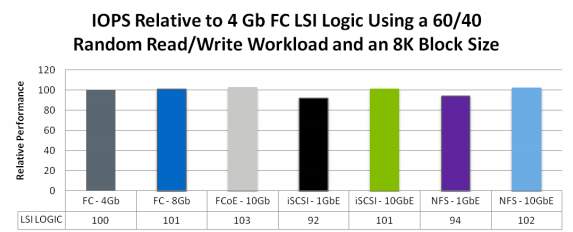
\includegraphics[width=\linewidth, keepaspectratio = true]{media/netapp_iops.png}
\mycaption{figure}{\label{abb:NetappIOPS}Netapp IOPS durchsatz für alle unterstützte Protokolle in Vergleich zu 4Gb FC mit 8K Block grösse\cite{Jafri2011}}
\end{center}

Der Report von Netapp hat ebenfalls die Latenz verglichen. Bei Latenz möchte man möglichst einen tiefen Wert erreichen. Gemäss \refabb{abb:NetappLatenz} ist die Latenz von iSCSI in einen 1 Gb Ethernet Netzwerk rund 9\% höher als bei Fibre Channel in einen 4Gb Netzwerk. Bei iSCSI in 10Gb Ethernet waren die Werte gleich wie Fibre Channel in 4Gb Netzwerk. Fibre Channel in einen 8Gb Netzwerk hatte jedoch rund 1\% tiefere Werte.\cite{Jafri2011}

\begin{center}
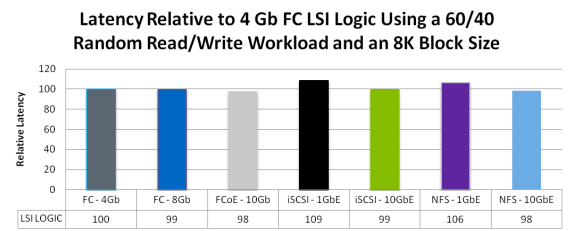
\includegraphics[width=\linewidth, keepaspectratio = true]{media/netapp_latence.png}
\mycaption{figure}{\label{abb:NetappLatenz}Netapp Latenz für alle unterstützte Protokolle in Vergleich zu 4Gb FC mit 8K Block grösse \cite{Jafri2011}}
\end{center}
 
\subsection{Logical Volume Manager}
Logical Volume Manager oder Dateisysteme welche die Logik eines Logical Volume Manager Kombinieren, ermöglichen es mehre Block-Geräte bzw. Logical Units zu einer grossen Logischen Volume zusammen zufassen. Diese hat den Vorteil, das die maximale Grösse eines Block-Gerätes nicht der limitierende Faktor des darauf installierten Dateisystems ist. Neben dem erstellen von Logischen Volume, können einige Logical Volume Manager den Last-Zugriff auf die verschiedenen Block-Geräte durch Striping optimaler verteilen und sorgen damit für eine besser Performance beim Datenzugriff. Eine weitere Aufgabe, die Logical Volume Manager übernehmen, ist die redundante Haltung der Daten durch Spiegelung. Mittel serverseitige Spiegeln (Host-Based Mirroring) können die Daten mittels der Spiegelungsfunktion des Logical Volume Manager auf zwei Standorte zur Verfügung gemacht werden. Dazu werden von zwei Speichersystemen, welche an unterschiedlichen Standorten installiert sind, gleich viele und gleich grosse Logical Units über das SAN dem Computersystem zugeteilt werden.

Klassische Server Linux Distributoren, wie Red Hat, Suse und Debian inkl. Ubuntu liefern den Quelloffenen Logical Volume Manager 2 (LVM2) in Ihrer Distribution mit. LVM2 kann theoretisch auf einen 64Bit System eine Logical Volume von 8 Exabyte bilden und adressieren.\cite{Levine2009}

Das ursprünglich von Oracle als ZFS Ersatz entwickelte Btrfs Dateisystem, könnte sich zukünftig als Standard Dateisystem vieler Server Distributionen entwickeln. Das für Solaris entwickelte ZFS als auch Btrfs kombinieren Dateisystem und Logical Volume Manager. Btrfs selbst wurde jedoch noch nicht als stabile Version veröffentlicht und ist deshalb für den produktiven Betrieb noch nicht zu empfehlen.\cite{Redler2011}


\subsection{Datei System}
Betriebssysteme adressieren die Daten auf einem Block-Geräte nicht direkt an, sondern greift über ein Dateisystem zu. Das Dateisystem organisiert wie und wo Dateien auf dem Block-Geräte abgelegt werden und Verwalten den freien Speicher. Einige Datei Systeme regeln auch die Zugriffsberechtigungen auf Dateien. Ein Block-Geräte (Logical Unit) können im SAN oder DAS an Mehren Computersysteme gleichzeitig zugeteilt werden, jedoch ist es die Aufgabe des Dateisystems sicherzustellen, dass mehre Computersysteme gleichzeitig auf das gleiche Dateisystem lesen bzw. schreiben können. Konventionelle Dateisysteme wie Ext3 unter Linux gehen von einer exklusiven Nutzung des Speichers aus, weshalb diese Dateisysteme keine Funktionen implementiert haben, die den gleichzeitigen Zugriff regeln. Problematik beim gleichzeitigen Zugriff ist die Sicherstellung der Konsistenz. Schreiben zum Beispiel zwei Computersysteme gleichzeitig in dieselbe Datei, kann nicht sichergestellt werden, welche Änderung gültig ist, und führt zu Inkonsistenz. Dateisysteme, welche den gleichzeitigen Zugriff von Mehren Computersysteme unterstützen, regeln den Zugriff auf Dateien mit Sperrmechanismen (locking). Schreibt ein Computersystem in eine Datei, wird die Datei vom Dateisystem vor der Änderung anderen Computersystem gesperrt. Cluster Dateisysteme wie Red Hat Global Filesystem (GFS) und Red Hat Global Filesystem 2 (GFS2) unterstützen dieses Sperren. Das Dateisystem Red Hat GFS Version 2 unterstützt bei einem 64-bit-System theoretisch Dateisysteme bis 8 Exabyte, Red Hat gewährleistet jedoch nur einen Support von maximal 100 Terabyte.\cite{Levine2011}

Dateisysteme wie ZFS und Btrfs stellen die Integrität der Daten vor Veränderung, wie Sie zum Beispiel durch ein Bit Fehler auf dem Block Geräte oder in Memory entstehen können, mittels Prüfsumme sicher. Dabei wir zur jeder Datei eine Hash Prüfsumme abgespeichert, wird die Datei gelesen wird die Prüfsumme aus der Datei neu berechnet und mit der abgespeicherten Prüfsumme verglichen, sofern das Dateisystem ebenfalls gespiegelt ist, korrigiert das Dateisystem die fehlerhafte Datei aus der intakten Kopie. Dieses Verfahren wird auch als Selbst heilend (Self-healing) bezeichnet. \cite{Bonwick2005}\cite{Oracle}

Dateisysteme können mittels Sicherungssoftware auf Bandlaufwerke oder andere Speichermedien gesichert werden.


\subsection{Zusammenfassung}


\section{Datei-Basierend}
Bei Datei basierte Speicherarchitekturen werden Daten nicht wie bei Block basierten Speicherarchitekturen über Blocke adressiert, sondern über Dateien.

Mit dem Aufkommen von Desktop-Computer, wurden die Daten nicht mehr Zentral auf einen Mainframe bearbeitet, sondern vermehrt verteilt auf den einzelnen Desktop-Computer. Ohne Vernetzung der Computer mussten die Daten mittels portablen Speichermedien ausgetauscht werden. Diese mag noch in kleinen Umgebungen praktikabel gewesen, sobald jedoch die Anzahl Teilnehmer steigt, wird es schwierig, den Überblick über seine Daten zu haben. Die reine Vernetzung der Computer und den direkten Austausch zwischen den einzelnen Desktop-Computer über eine Netzwerk bietet hier ebenfalls keine Lösung. Die bessere Lösung dieses Problems ist eine Zentraler Speicher in welcher die Dokumente (Dateien) gespeichert sind und mittels Netzwerk Protokoll den Desktop-Computer zur Verfügung gestellt werden. Somit ist es für den Anwender klar welche Dateien existieren und hat zugriff auf auf die aktuelle Version. Unternehmen wie Sun Microsystem, IBM, Microsoft und Apple erkannten ebenfalls dieses Bedarf und entwickelten für Ihre Betriebsysteme Software und dazugehörige Protokolle für den geteilten Datenzugriff.

Zu den bekanntesten und weitverbreitesten Lösungen zählen NFS und CIFS (SMB).


\subsection{Network File System}
Das ursprünglich rein von der Firma SUN Microsystems (heute Oracle) 1984 entwickeltes Network-File-System, ermöglicht den gemeinsamen Zugriff von mehreren Computersystemen auf das Dateisystem eines anderen Host (Server), als ob er zugriff auf ein lokales Dateisystem stattfindet. Die zweite Version von NFS erschien 1989 und war die erste Version welche von Internet Standard Request for Comments (\gls{RFC}) Standardisiert wurde und unter der RFC Nummer 1094 \footnote{003c?dpf /orth ?&gt;{http://tools.ietf.org/html/rfc1094}} veröffentlicht wurde. Für den Transport des NFS Protokoll wurde bis Version zwei ausschliesslich das \gls{UDP} Transportprotokoll unterstützt.
Die Version 3 von NFS (RFC 1813)\footnote{003c?dpf /orth ?&gt;{http://tools.ietf.org/html/rfc1813}}, die 1995 veröffentlicht wurde, war die erste Version, welche Maschinen, Betriebsystem und Netzwerk Architektur, und Transport-Protokoll unabhängig ist. Die Unabhängigkeit wird mit der Verwendung von Remote Procedure Call (\gls{RPC}), welches wiederum ein eXternal Data Representation (\gls{XDR}) verwendet, erreicht. \cite{Stern2001}

Wie im \refabb{} zu entnehmen ist, ist NFS eine weitere Schicht, welche auf dem Dateisystem und dessen Block-Geräte des Computersystems bzw. Speichersystem aufbaut. So ist es zum Beispiel die Aufgabe des Dateisystems bzw. des Block-Gerätes sich um die Redundanz und Integrität der gespeicherten Daten zu kümmern. 

Die Konsistenz der Daten, bei gleichzeitigem Zugriff von Mehren Computersysteme, stellt NFS mit einem separaten Protokoll, genannt Network Lock Manager (NLM) sicher. Der Network-Lock-Manager sorgt dafür, dass eine Datei, welche von einem Computersystem geändert wird, vor der Änderung anderen Computer Systeme gesichert ist. Wenn ein Client eine Sperrung angefordert hat, muss der Client, nach nicht mehr gebrauch der Sperrung, dem Server die Entsperrung mitteilen. Dieser Implementierung der Sperrung führt jedoch zu Problemen, wenn der Client ein System Absturz erleidet, in diesen Fall kann der Client die Entsperrung dem Server nicht mitteilen und die Datei bleibt für gesperrt.
NFS setzt mit NLM das Advisory Locking Sperr-Verfahren ein, dass bedeutet, dass ein weiter Client beim Zugriff auf eine gesperrte Datei nur hingewiesen wird, dass die Datei gesperrt ist, aber nicht den Client zwingt, keine Änderung vorzunehmen.\cite{Stern2001}


Seit Version 4 von NFS Protokoll (RFC 3530) ist das Sperre-Verfahren (Locking) im Protokoll selber implementiert, dadurch entfällt der zusätzliche Einsatz von Network Lock Manager. NFS Version 4 beherrscht das Sperren von Bytes-Bereich in einer Datei. Zudem erhält der Client von Server nur einen Leasing-Zeitraum für eine Sperrung (Lock), welcher er vor Ablauf wieder erneuern muss, um die Sperrung aufrecht zu halten. NFS in der Version 4 unterstützt das Sperr-Verfahren Mandatory Locking, dass bedeutet ein weiter Client kann, sich über die Sperrung nicht hinwegsetzen.\cite{Callaghan2003}

Dadurch, dass NFS auf TCP/IP als Kommunikation Protokoll aufbaut, kann eine NFS Freigabe, Standort übergreifend verfügbar gemacht werden, jedoch gilt auch hier das die Latenz und die Bandbreite der Verbindung zwischen den Standorten der limitierende Faktor ist.

NFS selbst hat keine eigene Implementierung für die Sicherstellung der Integrität der übermittelten Daten, stattdessen verlässt sich NFS seit Version 2 auf TCP und Ethernet Fehler Erkennung. TCP prüft im Standard verfahren die Integrität mit einer 16-Bit-Integer Prüfsumme. Die 16-Bit-Integer Prüfsumme erkennt Fehler im pseudo IP-Header, TCP-Header und Daten. Das Verfahren hat jedoch schwächen bei Einzel Bit-Fehlern Erkennung. Ethernet verwendet für die Fehlererkennung einen CRC32 Prüfsumme, diese gilt als effektive in der Erkennung Behebung von Bit Fehler, bietet aber keine durchgehend (End-to-End) Schutz. Grund dafür ist, dass beim Wechseln des Pakets der Kollisionsdomäne, wie es bei einen Swtich oder Router der Fall ist, jedes Mal eine neu CRC32 Prüfsumme erstellt wird.\cite{JohnL.202}. Bei NFS ab Version 4 kann der Datentransfer zusätzlich mit Kerberos abgesichert werden. Kerberos hat einen strengen Schutz gegen Manipulationen am Datenpaket und stellt somit die Integrität der Daten sicher. Nachteil ist aber das Kerberos zusätzlich eingerichtet werden muss. 

Bis und mit Version 4, wahren die Verarbeitung der Metadaten und die Verarbeitung der Daten in einem Protokoll und Server implementiert. NFS skalierte deshalb bis anhin bei der Verarbeitung von Dateien mit grosser Speicherplatz bedarf nicht ausreichend. Fragt einen NFS Client einen NFS Server für eine Datei an prüft der Server die Metadaten, die Metadaten enthalten den Speicherort, die Grösse, das Erstellungsdatum und das Änderungsdatum einer Datei, und wandelt die Anfrage in einen Disk I/O um, die Daten der Datei werden gesammelt und über das Netzwerk übertragen. Bei kleinen Dateien verwendet der Server die meiste Zeit für das sammeln der Daten, bei Grössen Dateien ist der limitierende Faktor der Transfer der Daten über das Netzwerk selbst.
Mit der Entwicklung von pNFS wurde der Transfer der Daten parallelisiert. Die Architektur von NFS wurde dazu in mehre Komponenten aufgeteilt. Der NFS Server besteht neu aus einen getrennten Metadaten Server und eine oder mehre Daten-Servern. Die Aufgabe des Metaservers ist die Verwaltung der Daten wo und wie die Daten gespeichert sind. Die Daten Servern, wo die Dateien gespeichert sind, kümmern sich um lese und schreib Anfragen von den Clients.
Bei einer anfrage an einer grosse Datei können Mehrere Daten-Server parallel Teile von der Datei dem Client ausliefern, der Client kann dann die Verschiedenen teile der Datei wieder zusammen setzen zu einer ganzen Datei. \cite{Shepler2010}\cite{Group2010}

Mit der NFS Version 4.1 wurde pNFS Bestandteil von NFS und ist seit 2010 im RFC 5661 standardisiert. Server Linux Distributoren, wie Red Hat haben allerdings NFS 4.1, erst als Vorschau in Ihrer Distribution integriert.\cite{EastJacquelynnMichaelHidep-Smith2011}




\subsection{NAS Appliance}

Network Attached Storage sind Speichersystem mit angepassten Datei System für den gemeinsamer Dateizugriff in einen Hetrogenen Computer Netzwerk welche über ein LAN angeschlossen sind. Als Speicher verwenden NAS je nach Typ interne Festplatten, Direct Attached Storage oder über eine SAN angefügten Speicher.
An Clients stellen NAS Ihren Speicher über NFS, CIFS, ISCSI zur Verfügung. High-End NAS können Ihren Speicher wiederum über Fibre-Channel zur Verfügung stellen.

Gemäss Gartner gehören die Anbieter IBM, EMC und NetAPP zu den führenden NAS Anbieter in Midrange und High-End bereich. Wobei gemäss Garnter Magic Quadrant Netapp zusammen mit EMC zu den innovativsten Anbieter.

\begin{quotation}
\em 
\textbf{Strengths}
\begin{itemize}
\item NetApp remains one of the few truly unified storage providers among all top-tier vendors, with its software features continuing to be industry benchmarks. The company was able to regain some of the NAS revenue market share that it had lost in 2009. Its fast revenue growth in 2010 was driven by its successful campaign targeted at midsize enterprises with the value propositions of NFS supporting VMware and unified storage in consolidating Windows application storage.

\item In 2010, NetApp increased its aggregate up to 100TB with Data ONTAP 8.0.1 and introduced compression to complement its popular deduplication capability. It added a RESTful object storage interface (based on its acquisition of Bycast) to its unified storage, targeting global content repositories. On the hardware side, it launched new systems with better performance and denser disk shelves.

\item NetApp's new software bundles have simplified the procurement process and made software pricing more affordable. For customers seeking converged infrastructure, NetApp launched FlexPod for VMware with its partners Cisco and VMware, offering packages including servers, storage and switches.
\end{itemize}
\textbf{Cautions} 
\begin{itemize}
\item The vast majority of the Data ONTAP 8.0 adoption was on the 7 mode (instead of the cluster mode) for larger aggregates, while the early adoption of the cluster mode focuses on high- performance NFS file services. The cluster mode is not ready for mainstream enterprise customers who require those 7-mode features that are still missing in the cluster mode. The ONTAP 8.1 scheduled for release later this year will likely continue to support the two modes: clustered and nonclustered modes of operation.
\item While NetApp continues to enjoy its leading edge in unified storage, it's facing fiercer competition in the high-end NAS market, where file systems larger than 100TB are required and where high performance without the expensive Flash Cache is desired.
NetApp is also challenged in the low-end NAS and unified storage market with new products from both major and emerging competitors.
\end{itemize}
\end{quotation}\cite{IEEE2003}



\subsection{Zusammenfassung}


\section{Objekt-Basierend}

\subsection{Verteilte Dateisysteme}
Unternehmen wie Google, welche Web-Applikationen mit Millionen von Anwendern Betreiben und der Speicherbedarf von hunderten Terrabyte bis Petabyte an Daten,  haben hohe Anforderungen an Ihr Speichersystem. Google hat für Ihren Bedarf eine eigenes Verteiltes Dateisystem genannt Google Filesystem entwickelt. Google hat beim Designe und des Dateisystem angenommen, das es auf gewöhnlichen und günsige Hardware laufen kann, welche aber öfter Komponenten Fehler habe. Daher ist der Ausfall von Komponenten nicht eine Sonderfalls sondern gehört zur Normalität. Zudem handelt sich bei den gespeicherten Dateien eher um grössere Dateien mit 100 Megabyte bis Multi Gigabyte an grösse. Die Auslastung ist primär durch zwei Arten von lese Vorgänge verursacht. Das lesen eines ganzen Datenstroms und das regellos Lesen. Die Schreibbelastung wird durch grosse Sequentiele schreib Vorgänge verursacht und Dateien werden erweitert als modifiziert. Als Architektur hat Google einen Cluster gewählt bestehend aus einen einzigen Metadaten Server und mehren Chunksserver. Die Daten werden bei Google in Einheiten genannt Chunks unterteilt und jeder Chunk bekommt eine eindeutige Identifizierung. Diese Chunks werden über mehre Chunkserver repliziert um die Ausfallsicherheit zu gewährleisten. Der Metadaten Server speichert in seinen Arbeitsspeicher die ganze metadaten bestehend aus Namensraum, Berechtigung Informationen, die Zuordnung der Datei zu den Chunks, und die Speicherort der Chunks. Google hat Ihre Dateisystem bis anhin nicht veröffentlich, hat jedoch eine  Studie über die Desinge und Architektur Prinzipen veröffentlicht. Einige erhältliche Verteileten Dateisysteme, wie Hadoop Distributed Filesystem (HDFS), CloudStore und GLORY-FS beruhen auf den selben Architektur Prinzipen aus der Studie.


 Diese Studie galt für eine Verteilte Dateisysteme, wie Hadoop Distributed Filesystem (HDFS), CloudStore, GLORY-FS,
 Das Google Filesystem 

welche die


 Google stellte an sein Dateisystem folgende Anforderungen: 
\begin{itemize}
\item Komponenten Fehler sind die Norm
\item Multi-Gigabyte Dateien sind häufig
\item Dateien werden werden hauptsächlich erweitert als überschrieben
\end{itemize}

Für diese Hauptanforderungen hat Google eine eigenes Dateisystem Entworfen und Entwickelt.


